

\section*{Houdini bascis}

\markboth{\hspace{1cm}workshop exercices}{RC11\hspace{1cm}}


word\footnote{Explanation of the word.} that Addjword\footnote{Explanation of the word.} thatjord\footnote{Explanation of the word.} thatYou can find the source code on GitHub: \url{https://github.com/your-username/your-repository}.


 \keywords{-5}{-4cm}{16cm}{node, houdini, procedural,Eproceduralism, attribute, geometry, vop, vex,}

dfddddFor the first exercise, a description of two  example exercises is needed.
go intro as much detail as possible. Think about keywords like : node, attribute, dataype, points, vertecis, primitives, parameter, classes, type.

A possible 



\begin{multicols}{2} 
some text here 
\lipsum[1-2]


	\begin{figure}[H]
	    \centering
		
		\noindent  
	    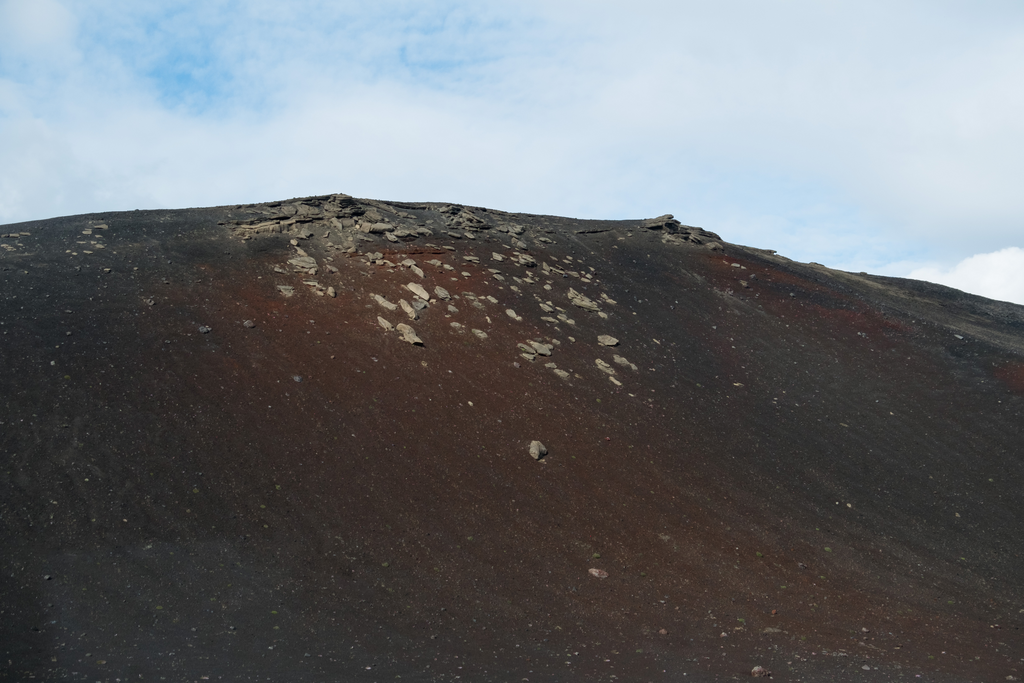
\includegraphics[width=\linewidth]{sections/assignment_1/t.png}
%	    \caption{Your caption here}
%	    \label{fig:example}
	\end{figure}
some texct here
\lipsum[1-2]
\end{multicols}

\lipsum[1-2]





































